\documentclass{article}
\usepackage{amsmath}
\usepackage{pgfplotstable}
\usepackage{graphicx}
\usepackage{subcaption}
\usepackage{verbatim}
\usepackage{amssymb}
\usepackage{hyperref}
\usepackage{float}

\title{Project 1 on Machine Learning: Regression analysis and resampling methods}
\author{Bj{\o}rn Gr{\o}nntun}
\DeclareMathOperator*{\argminA}{arg\,min}
\begin{document}
\maketitle
\begin{abstract}
    In this report, we will examine how regression techniques can be used to predict quantitative data. The data with which we will be working are partly generated, partly real world geographical data. The Ordinary Least Squares method goes back at least to the great Gauss, and will provide the backbone for all the techniques we discuss. Among other things, we will see how input data may be transformed, giving rise to models that, although non-linear with respect to the original data, behave exactly as linear models. We will also consider methods for evaluating how well our models generalize to unseen data, leading to a theoretical discussion of the so-called bias-variance tradeoff. Ridge and Lasso regression are also introduced, both being modifications to the original Ordinary Least Squares method that may help reducing the generalization error in some cases.
\end{abstract}
\section*{Some words on project structure}
The entire project can be found at \url{https://github.com/bjorngronntun/FYS-STK4155-project1}. The main project folder contains the following subfolders:
\begin{description}
    \item[data] - containing both raw and data processed or generated during the course of the project
    \item[notebooks] - containing Jupyter notebooks, representing the "experimental phase" of the project
    \item[reports] - containing this final report along with figures and csv files therein displayed
    \item[src] - containing Python modules
\end{description}

Although this report summarizes every result obtained, the reader is invited in particular to browse the notebooks, where he or she may follow in detail how the results were obtained. The notebooks represents the gradual evolution of the project in its entirety. Everything is meant to be reproducible - if the reader chooses, he or she can delete the files in \texttt{data/generated}, \texttt{reports/csv\_files} and  \texttt{reports/figures} and use the notebooks to recreate them. In that case, the following "natural ordering" of the notebooks should be respected:

\begin{enumerate}
    \item \texttt{20190920-Generating-Franke-data.ipynb}
    \item \texttt{20190905-visualizing-franke.ipynb}
    \item \texttt{20190906-OLS-Franke.ipynb}
    \item \texttt{20190918-Resampling-OLS-Franke.ipynb}
    \item \texttt{20191002-Training-versus-test-error-plot-OLS.ipynb}
    \item \texttt{20190928-Ridge-regression-Franke.ipynb}
    \item \texttt{20191005-Lasso-regression-Franke.ipynb}
    \item \texttt{20190907-introducing-terrain-data.ipynb}
\end{enumerate}

Of course, the reader may also peruse the actual Python modules in the $\texttt{src}$ folder. The modules contain unit tests - the testing is briefly described in the special notebook \texttt{20190906-testing.ipynb}.

\section{Ordinary Least Squares on the Franke Function}
When building and analyzing our models, it makes sense to have some simple data to test them on. In this section, we will generate our target values by sampling the Franke Function on the unit square. This function, which is widely used when testing interpolation and fitting algorithms, is given by

\begin{align*}
    f(x, y)
    &={\frac{3}{4}\exp\left(-{\frac{(9x-2)^2}{4}} -{\frac{(9y-2)^2}{4}}\right)}\\
    &+{\frac{3}{4}\exp\left(-{\frac{(9x+1)^2}{49}}-{\frac{(9y+1)^2}{10}}\right)}\\
    &+{\frac{1}{2}\exp\left(-{\frac{(9x-7)^2}{4}}-{\frac{(9y-3)^2}{4}}\right)}\\
    &-{\frac{1}{5}\exp\left(-{(9x-4)^2}-{(9y-7)^2}\right)}
\end{align*}
It should be noted right away that even if the Franke function is exponential in $x$ and $y$, Taylor's theorem should guarantee that we will be able to get quite close to the original Franke data by using fifth-degree polynomials. In addition to the "pure" Franke values given by the function, we will generate a couple of perturbed variations by adding normally distributed noise. This will give us the opportunity to study how it will be more difficult to create a good fit to the data as it grows more complex.
\subsection{Generating and visualizing data}
The Franke data are generated in the notebook \texttt{20190920-Generating-Franke-data.ipynb}, which relies on \texttt{src/data/generate\_data.py}. By varying the noise term, we get three sets of target values, which are stored in separate files:
\begin{itemize}
    \item \texttt{no\_noise.csv} with no noise added to the Franke data
    \item \texttt{some\_noise.csv}, where normally distributed noise with mean 0 and standard deviation 0.1 is added to the Franke data
    \item \texttt{noisy.csv}, where normally distributed noise with mean 0 and standard deviation 0.4 is added to the Franke data
\end{itemize}
The data are stored in \texttt{data/generated/}. Of course, the data could easily have been generated on the fly as needed, but by storing it at this point, we facilitate reproducibility, as we do not run the risk of generating lots of datasets that may look similar, but actually are different from each other. From this point on, we will work with the data read from the files, and nothing else.

In the same notebook (\texttt{20190920-Generating-Franke-data.ipynb}) we also generate a feature matrix $X$. In addition to the original grid points $\{(x=0.05i, y=0.05j): i, j = 0, ..., 19\}$ we include features of the form $x^m y^{n}$, where $m$ and $n$ are non-negative integers and $m+n \leq 5$. This is in order to perform polynomial regression analysis, which is just another name for ordinary linear regression performed on a feature matrix augmented by polynomial combinations of the original features. The heavy lifting in constructing the polynomial features is performed by the class \texttt{PolynomialFeatures} in \texttt{src/features/polynomial.py}. Again, we choose to store the generated feature matrix for subsequent use (\texttt{data/generated/X.csv}).

We now have one common feature matrix and three different sets of target values. In the notebook \texttt{20190905-visualizing-franke.ipynb}, we perform some simple exploratory data analysis on those datasets. The table below shows the output of the \texttt{describe} function from \texttt{pandas}\footnote{I have saved the output into the file \texttt{1\_description\_table.csv} and load it into \LaTeX using the \texttt{pgfplotstabletypeset} package, but as my \LaTeX skillset is somewhat limited, it shows up strangely - I am not able to display the percentage signs in the row names of the percentile rows.}.

\begin{table}[h]
    \pgfplotstabletypeset[
        col sep=comma, ignore chars={, \%},
        every head row/.style={
            before row={
                \hline
            },
            after row=\hline
        },
        every last row/.style={
            after row=\hline
        },
        columns/{0}/.style={column name=, string type}
    ]{csv_files/1_description_table.csv}
    \label{tab:description}
    \caption{Description of target data}
\end{table}

The table gives us some insight into the difference between the three sets of target values, in particular when we look at the spread (compare the standard deviation and the difference between the max and min rows.)

We can also get a feel of the data by plotting them. The code for the following contour plots is in the notebook \texttt{20190905-visualizing-franke.ipynb}. We see that the original Franke function seems quite smooth, whereas the noisy version is full of "spikes" that will make fitting harder.


\begin{figure}[h!]
    \centering
    \begin{subfigure}{0.6\linewidth}
        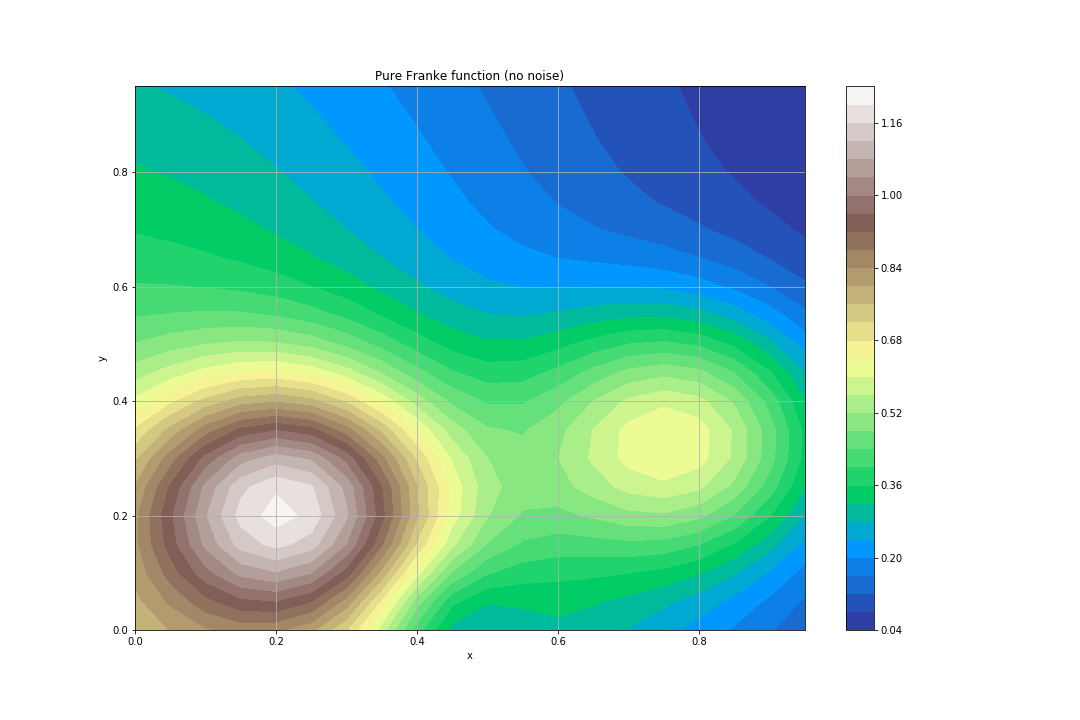
\includegraphics[width=\linewidth]{figures/1_franke_contour_no_noise.png}
        \caption{No noise}
    \end{subfigure}
    \begin{subfigure}{0.6\linewidth}
        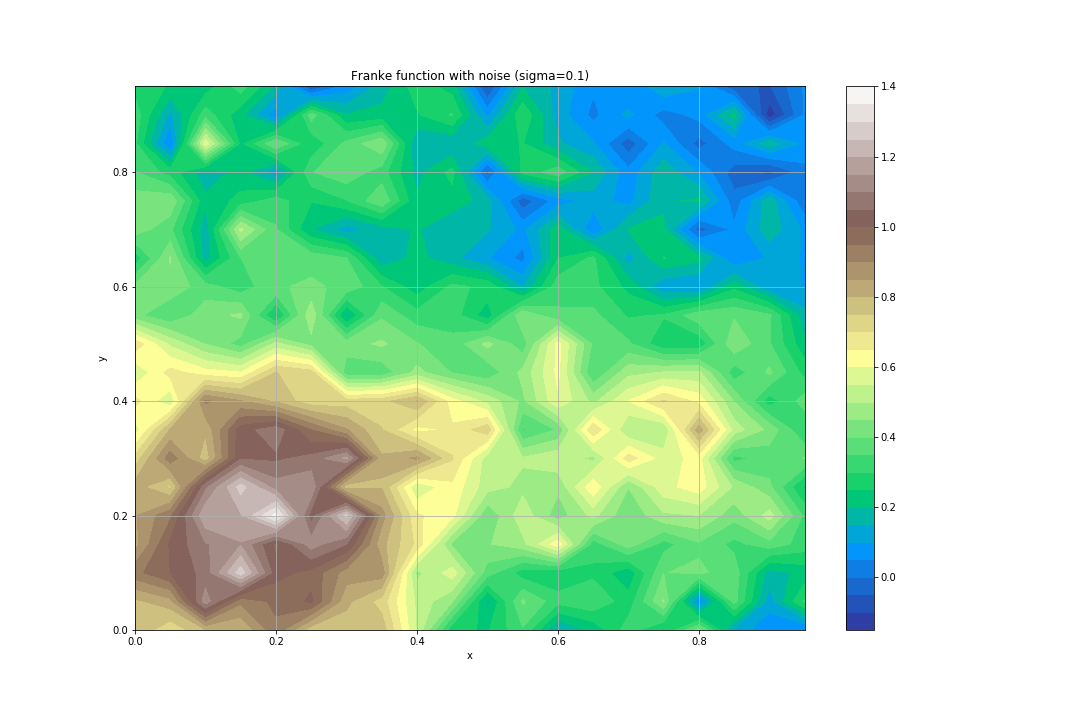
\includegraphics[width=\linewidth]{figures/1_franke_contour_some_noise.png}
        \caption{Some noise (sigma=0.1)}
    \end{subfigure}
    \begin{subfigure}{0.6\linewidth}
        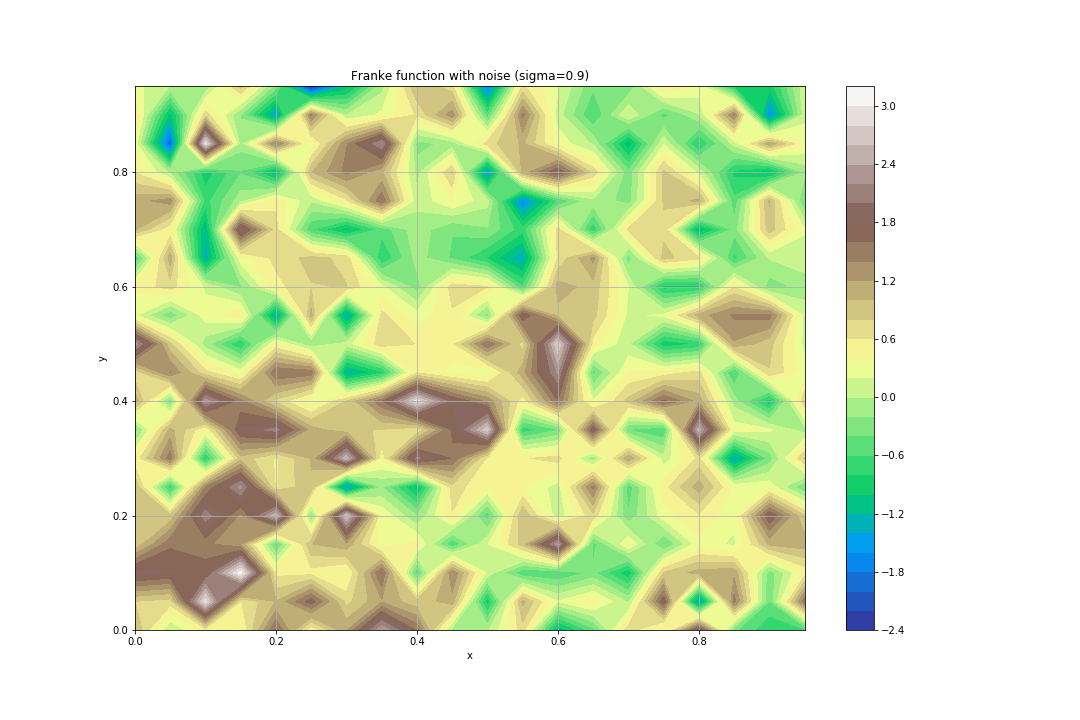
\includegraphics[width=\linewidth]{figures/1_franke_contour_noisy.png}
        \caption{Noisy (sigma=0.4)}
    \end{subfigure}
    \caption{Franke functions contour plots}
\end{figure}


\subsection{Ordinary Least Squares regression - theoretical recap}
\subsubsection{Function fitting}

We now proceed to actually fitting functions to the data points. The OLS (Ordinary Least Squares) method is very well known, so the following description will be brief. Given data points $\{(x_i, y_i): i=1, ..., m\}$, where each $x_i$ is a vector in $\mathbb{R}^n$ and each $y_i$ is a real number, we want to obtain a parameter vector $\hat{\beta}\in\mathbb{R}$ so that for each input vector $x_i$, the predicted output $\hat{y_i}={x_i}^T \hat{\beta}$ will be "close to" the target value $y_i$. One possible way to do this is to choose $\hat{\beta}$ so as to minimize the sum of squared errors, that is, to set

$$
\hat{\beta} = \argminA_{\beta} \sum_{i=1}^{m}{(y_i - {x_i}^T \beta)^2}
$$

If we collect the $(x_i)$ in a feature matrix

$$
\mathbf{X} =
\begin{bmatrix}
    {x_1}^T \\
    {x_2}^T \\
    \hdotsfor{1} \\
    {x_m}^T
\end{bmatrix}
$$

we easily see that the above minimization problem can be formulated as

$$
\hat{\beta} = \argminA_{\beta} \left\|\mathbf{y - X\beta}\right\|^2
$$

The minimization problem turns out to have a closed form solution, which can be found using matrix differentiation. The solution is

$$
\hat{\beta} = ({\mathbf{X}}^T \mathbf{X})^{-1} {\mathbf{X}}^T \mathbf{y}
$$

Of course, this solution only exists if ${\mathbf{X}}^T \mathbf{X}$ is nonsingular, but this is rarely a problem in real-life situations. There are more effective ways of computing the least-squares estimate for $\beta$, but we stick to matrix inversion here, as it is very easy to implement. The implementation is in the $\texttt{fit}$ method of the $\texttt{OLS}$ class in $\texttt{src/models/models.py}$.

\subsubsection{Estimates of error and variability}

Once we have obtained our estimates for $\beta$, we can get predictions $\mathbf{\hat{y}}$ by putting $\mathbf{\hat{y}} = \mathbf{X}\hat{\beta}$. We then can assess the quality of our estimates in various ways. The MSE (Mean Square Error) is one such measure. Given target values $\mathbf{y}$ and predictions $\mathbf{\hat{y}}$, the MSE is given by $\frac{1}{m}\left\|\mathbf{y - \hat{y}}\right\|^2$. The implementation of the MSE is in $\texttt{src/evaluation/evaluation.py}$, along with a function for evalutating the $R^2$ score. The $R^2$ score measures how much the error is reduced by using our linear model as opposed to a pure mean model, that is, a model where we predict $\hat{y_i} = \frac{1}{m}\sum_{i=1}^{m}{y_i}$ for $i=1, ..., m$. The ratio between the mean square errors of the two models is

$$
\frac{ \sum_{i=1}^{m}{(y_i - \hat{y_i})^2}}{ \sum_{i=1}^{m}{(y_i - \bar{\mathbf{y}})^2}}
$$

where $\bar{\mathbf{y}} = \frac{1}{m}\sum_{i=1}^{m}{y_i}$. We want this ratio to be low, that is, we want our model predictions to be much better than the values predicted by the pure mean model. This leads us to defining an measure

$$
R^2
= 1 -
\frac{ \sum_{i=1}^{m}{(y_i - \hat{y_i})^2}}{ \sum_{i=1}^{m}{(y_i - \bar{\mathbf{y}})^2}}
$$

which will hopefully be close to 1.

The last measure we are going to discuss is the variance of our estimates for $\beta$. This is an important issue, because when doing linear regression, we assume a "ground truth" model $y_i = {x_i}^T\beta + \epsilon$, where the $\epsilon$ is a normally distributed random variable. This means that $\mathbf{\hat{\beta}}$ is a random variable too, and we are interested in its variance, which will allow us to construct condifence intervals around our point estimates. It can be shown that the covariance matrix of $\hat{\beta}$ is ${\sigma}^2 ({\mathbf{X}}^T \mathbf{X})^{-1}$, where ${\sigma}^2$ is the variance of ${\epsilon}$. Because we are mainly interested in the variance of the individual components of $\hat{\beta}$, we focus on the diagonal of this matrix, and find that $\mathrm{Var}(\hat{\beta_j}) = {\sigma}^2 (({\mathbf{X}}^T \mathbf{X})^{-1})_{j, j}$. In general, ${\sigma}^2$ will be unknown to us, but it can be estimated by the MSE we calculated previously. This leads to the expression

$$
{\hat{\sigma}}^2 (\hat{\beta_j}) = \mathrm{MSE} \times (({\mathbf{X}}^T \mathbf{X})^{-1})_{j, j}
$$

as our estimate of the variance of $\hat{\beta_j}$\footnote{Have I misunderstood anything here? According to the lecture note, the square root of $(({\mathbf{X}}^T \mathbf{X})^{-1})_{j, j}$ should be taken in this formula, but this does not seem right.} Having obtained variance estimates, we can take their square root ${\hat{\sigma}}_{\hat{\beta_j}}$ and construct 95 \% confidence intervals as

$$
\left[ {\hat{\beta_j}} - 1.96{\hat{\sigma}}_{\hat{\beta_j}}, {\hat{\beta_j}} + 1.96{\hat{\sigma}}_{\hat{\beta_j}} \right]
$$

\subsection{Ordinary Least Squares regression - results}
In the notebook $\texttt{20190906-OLS-Franke.ipynb}$, we perform OLS regression on our generated datasets and evaluate our results using the metrics described above. This notebook depends upon $\texttt{src/models/models.py}$ for the actual data fitting and $\texttt{src/evaluation/evaluation.py}$ for the metrics. We begin by comparing the output from the regression method with the target values of the three datasets, and obtain the following results:

\begin{table}[h]
    \pgfplotstabletypeset[
        col sep=comma, ignore chars={, \%},
        precision=5,
        every head row/.style={
            before row={
                \hline
            },
            after row=\hline
        },
        every last row/.style={
            after row=\hline
        },
        columns/{0}/.style={column name=, string type}
    ]{csv_files/1_mse_r2_score.csv}
    \caption{MSE and $R^2$ (no resampling)}
\end{table}

As we see, the $R^2$ scores are quite close to one in the pure Franke case, meaning that our model explains most of the variability in the data. In the more noisy datasets, the $R^2$ is much worse. The MSE, as expected, grows significally with added noise. A fifth-degree polynomial can be fitted rather well to a pure Franke function, whereas with added noise, the fitting becomes much harder.

We now proceed to the actual parameter estimates and their variances. Because we have three datasets and there are 21 parameters, we get quite a lot of data here. In the notebook $\texttt{20190906-OLS-Franke.ipynb}$ we construct three csv files corresponding to the three datasets. For the no-noise case, we get the following data:

\begin{table}[H]
    \pgfplotstabletypeset[
        columns={Feature, Estimate, Variance, {Lower bound}, {Upper bound}},
        col sep=comma,
        ignore chars={, \%},
        precision=5,
        every head row/.style={
            before row={
                \hline
            },
            after row=\hline
        },
        every last row/.style={
            after row=\hline
        },
        columns/Feature/.style={string type}
    ]{csv_files/1_parameters_with_confidence_intervals_no_noise.csv}
    \caption{$\beta$ estimates, no noise}
\end{table}

This table shows the $\beta$ estimates for each individual feature, along with the estimates for the variance and the lower and upper bound for the corresponding confidence intervals.

For the case where normally distributed noise with $\sigma=0.1$ is added to the output from the Franke function, we get the following parameter estimates and confidence intervals:

\begin{table}[H]
    \pgfplotstabletypeset[
        columns={Feature, Estimate, Variance, {Lower bound}, {Upper bound}},
        col sep=comma,
        ignore chars={, \%},
        precision=5,
        every head row/.style={
            before row={
                \hline
            },
            after row=\hline
        },
        every last row/.style={
            after row=\hline
        },
        columns/Feature/.style={string type}
    ]{csv_files/1_parameters_with_confidence_intervals_some_noise.csv}
    \caption{$\beta$ estimates, some noise ($\sigma=0.1$)}
\end{table}

Finally, for the case where normally distributed noise with $\sigma=0.4$ is added, we get this table:

\begin{table}[H]
    \pgfplotstabletypeset[
        columns={Feature, Estimate, Variance, {Lower bound}, {Upper bound}},
        col sep=comma,
        ignore chars={, \%},
        precision=5,
        every head row/.style={
            before row={
                \hline
            },
            after row=\hline
        },
        every last row/.style={
            after row=\hline
        },
        columns/Feature/.style={string type}
    ]{csv_files/1_parameters_with_confidence_intervals_noisy.csv}
    \caption{$\beta$ estimates, noisy ($\sigma=0.4$)}
\end{table}

The information that can immediately be gleaned from these three tables is that as the noise increases, the confidence intervals become progressively wider. (A plot should probably be inserted here.)

\section{Resampling techniques, adding more complexity}
Hitherto, we have evaluated our results using the same data we used for model fitting. In most real-life scenarios, this is considered bad practice, as the models tend to "learn" noise in addition to the underlying distribution of the data. Thus, we easily end up with models that are able to reproduce the original data quite well, but do not necessarily deal equally well with "unknown" data. This is known as the overfitting problem.

In order to get a better picture of how well our models generalize to unseen data, we can use different resampling techniques. One such approach is to split our data into two parts, known as the test set and the training set. We use the training set for model fitting and the test set for evaluation. As the test set consists entirely of unseen data, this gives us a much better understanding of the generalizing ability of the model.

In the notebook $\texttt{20190918-Resampling-OLS-Franke.ipynb}$ we use the function $\texttt{train-test-split}$ from $\texttt{sklearn.model\_selection}$ in order to achieve such a split. When evaluating our model's ability to reproduce the test data after having been trained on the training data, we get the following MSE and $R^2$:

\begin{table}[h!]
    \pgfplotstabletypeset[
        col sep=comma, ignore chars={, \%},
        precision=5,
        every head row/.style={
            before row={
                \hline
            },
            after row=\hline
        },
        every last row/.style={
            after row=\hline
        },
        columns/{0}/.style={column name=, string type}
    ]{csv_files/2_mse_r2_score.csv}
    \caption{MSE and $R^2$ using train-test-split}
\end{table}

If we compare this table to the corresponding table we made earlier, we see that the MSE is higher, in particular in the noisy case (0.209 versus 0.152). This is of course to be expected, as we now test our model on unseen data. The $R^2$ scores are visibly lower than before.

Resampling can be done in other ways as well. One possible approach is k-fold cross-validation, where we start by partitioning our data ${\mathcal{D}}$ into $k$ disjoint folds ${\mathcal{D}}_1, {\mathcal{D}}_2, ..., {\mathcal{D}}_k$. For $j=1, ..., k$, we then use ${\mathcal{D}}\setminus{\mathcal{D}}_j$ as our training set and ${\mathcal{D}}_j$ as our test set. For each value of $j$, we can obtain a MSE score, and by averaging the MSE scores, we hopefully get a precise estimate of the true MSE.

In the same notebook ($\texttt{20190918-Resampling-OLS-Franke.ipynb}$) we use the class $\texttt{K\_fold\_splitter}$ from $\texttt{src/resampling/resampling.py}$ to estimate the test MSE using cross-validation. We obtain the following results on our three datasets:

\begin{table}[h!]
    \pgfplotstabletypeset[
        col sep=comma, ignore chars={, \%},
        precision=5,
        every head row/.style={
            before row={
                \hline
            },
            after row=\hline
        },
        every last row/.style={
            after row=\hline
        },
        columns/{0}/.style={column name=, string type}
    ]{csv_files/2_cross_val_mse.csv}
    \caption{MSE scores using k-fold cross-validation}
\end{table}

These scores are somewhat lower than the ones we obtained using train-test-split. This is probably related to the size of the test sets - when doing train-test-split, our training sets contained only 70 \% of the instances, whereas when using 10-fold cross-validation, our training sets will contain 90 \% of the instances. In this case, the increased training set size seems to lead to some improvement of the MSE, but this may not always be the case, and should probably be investigated further.

\section{Bias-variance tradeoff}
Above we mentioned the importance of validating our models on unseen data in order to avoid overfitting. In this section, we will bring this somewhat "intuitive" idea onto a more precise theoretical footing. In particular, we will decompose our test MSE into three separate terms, of which the first may be interpreted as error stemming from adopting too rigid a model, which may not be able to capture the relevant fluctuations in the training set properly. This is called the bias (or to be more precise, the square of the bias). An obvious way to reduce the bias is to adopt a more flexible model, but this may easily introduce a second kind of error, which is the one described above, i. e. that the model fits too closely to the training set, picking up fluctuations due to sampling rather than to the true underlying distribution of the data. This second kind of error is known as variance.

As stated above, we take as our point of departure a dataset $\{(x_i, y_i): i=1, ..., m\}$ and a "ground truth" model $\mathbf{y} = f(x) + \mathbf{\epsilon}$. Hitherto, the function $f$ has been of the linear form $f(x) = {x}^T \beta$, but in the following discussion we will consider general models of this type. What is important is that the noise term $\mathbf{\epsilon}$ is normally distributed with mean 0 and variance ${\sigma}^2$.

When doing regression analysis, our goal is to obtain a model $\hat{f}$ to obtain predictions $\hat{\mathbf{y}} = \hat{f}(x)$. In this setting, both $\mathbf{y}$, $\mathbf{\hat{y}}$ and $\mathbf{\epsilon}$ are random variables. We have already stated that $\mathbb{E}{(\epsilon)}=0$ and $\mathrm{Var}{(\epsilon)} = {\sigma}^2$, and now proceed to compute the expectations and variances of $\mathbf{y}$ and $\mathbf{\hat{y}}$. To unclutter notation, we put $f=f(x)$, and note that since $f$ is deterministic, its expected value is $f$ and its variance is zero. We have

\begin{align*}
    \mathbb{E}{(\mathbf{y})}
    &=  \mathbb{E}({f + \mathbf{\epsilon}}) \\
    &= \mathbb{E}{(f)} + \mathbb{E}{(\mathbf{\epsilon})} \\
    &= f
\end{align*}
and
\begin{align*}
    \mathrm{Var}(\mathbf{y})
    &= \mathbb{E}[(\mathbf{y} - \mathbb{E}(\mathbf{y}))^2] \\
    &= \mathbb{E}[(f+\epsilon-f)^2] \\
    &= \mathbb{E}[(\epsilon - 0)^2] \\
    &= \mathrm{Var}(\epsilon) \\
    &= \sigma^2
\end{align*}

When doing regression analysis, we try to minimize the test MSE, which can be written as $\mathbb{E}[(\mathbf{y} - \mathbf{\hat{y}})^2]$. We can rewrite this in the following way. We set $u=\mathbb{E}(\hat{\mathbf{y}})$, again in an attempt to unclutter notation somewhat.

\begin{align*}
    \mathbb{E}[(\mathbf{y} - \mathbf{\hat{y}})^2]
    &= \mathbb{E}[(f + \epsilon - \mathbf{\hat{y}})^2] \\
    &= \mathbb{E}[(f + \epsilon - \mathbf{\hat{y}} + u - u)^2] \\
    &= \mathbb{E}[((f - u)
    + \epsilon
    + (u - \mathbf{\hat{y}}))^2] \\
    &= \mathbb{E}[(f - u)^2
    + {\epsilon}^2
    + (u - \mathbf{\hat{y}})^2
    + 2\epsilon(f - u)
    + 2\epsilon(u - \mathbf{\hat{y}}) + 2(f - u)(u - \mathbf{\hat{y}})] \\
    &= \mathbb{E}[{(f - u)^2}]
    + \mathbb{E}[{{\epsilon}^2}]
    + \mathbb{E}[{(u - \mathbf{\hat{y}})^2}]
    + \mathbb{E}[{2\epsilon(f - u)}]
    + \mathbb{E}[{2\epsilon(u - \mathbf{\hat{y}})}]
    + \mathbb{E}[{2(f - u)(u - \mathbf{\hat{y}})}] \\
    &= (f - u)^2
    + {\sigma}^2
    + \mathrm{Var}(\mathbf{\hat{y}})
    + 0
    + 0
    + 0 \\
    &= (f - \mathbb{E}(\mathbf{\hat{y}}))^2
    + \mathrm{Var}(\mathbf{\hat{y}})
    + {\sigma}^2 \\
    &= \frac{1}{m}\sum_{1}^{m}{(f_i - \mathbb{E}(\mathbf{\hat{y}}))^2}
    + \frac{1}{m}\sum_{1}^{m}{({\hat{y}}_i - \mathbb{E}(\mathbf{\hat{y}}))^2}
    + {\sigma}^2 \\
\end{align*}

The first of these terms is the square of the bias, which can be explained as the error resulting from erroneous assumptions in the learning algorithm, for instance that we assume a linear model when the actual underlying distribution is non-linear. The second term is the variance, which is the error resulting from our model picking up and incorporating randomness in the training set due to sampling. The last term is the irreducible error, stemming from the fact that the true underlying model $\mathbf{y} = f(x) + \mathbf{\epsilon}$ has a random noise term.

As the complexity of our model increases, it will more easily adapt to fluctuations in the training set. Thus while the bias decreases, the variance usually increases. This leads to an interesting trade-off situation: If we choose too simple a model, we will not be able to pick up important underlying patterns in the data, thus increasing our test MSE. However, if we make our model too complex, it will model noise in the training data, again increasing the test MSE.

In the notebook \texttt{20191002-Training-versus-test-error-plot-OLS.ipynb}, we try out polynomial models of degrees 0, 1, 2, 3, 4 and 5 on the noisy dataset. Thus we increase model complexity, and should expect a monotonically decreasing train MSE, whereas the test MSE could in principle increase. We obtain the following plot:

\begin{figure}[H]
    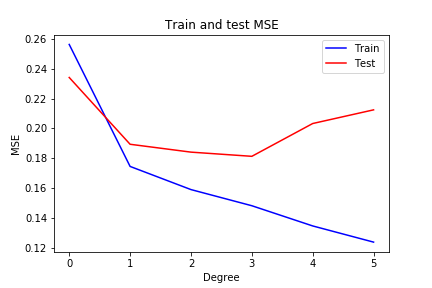
\includegraphics{figures/3_train_and_test_mse.png}
    \caption{Train and test MSE, noisy data}
    \label{}
\end{figure}

We clearly see that in this particular case, we seem to reach a "sweet spot" around degree 3, where the test MSE is optimal. Of course, further testing should be conducted in order to find out if this is a general tendency.

\section{Ridge regression on the Franke function with resampling}
As described above, we have fitted our OLS model parameters by minimizing the sum of squared errors on the training set. That is, we have solved the minimization problem

$$
\hat{\beta} = \argminA_{\beta} \left\|\mathbf{y - X\beta}\right\|^2
$$

The idea behind ridge regression is to introduce a penalty term that will "dampen" the obtained parameters somewhat by bringing them closer to zero. The minimization problem now becomes

$$
\hat{\beta} = \argminA_{\beta} \left\|\mathbf{y - X\beta}\right\|^2 + \lambda\left\|\beta\right\|^2
$$

Here, $\lambda$ is a non-negative real number. If $\lambda=0$, we get our usual OLS cost function. Higher values of $\lambda$ corresponds to more significant "damping" or regularization. As we have already stated that our original OLS approach has a closed-form solution that minimizes the sum of squared errors on the training set, we cannot expect our new approach to obtain a better result on the training set. This, however, is not really a problem, since we are interested in are models that perform well on unseen data, not on the same data as it was trained on. Our hope is that as we increase the bias slightly by forcing the $\beta$ parameters closer to zero, we reduce the variance so that the model will be less prone to overfitting. Hopefully, this will lead to a lower test MSE.

It can be shown, using matrix differentiation, that the Ridge regression minimization problem has a closed-form solution

$$
\hat{\beta} = ({\mathbf{X}}^T \mathbf{X} + \lambda\mathbf{I})^{-1} {\mathbf{X}}^T \mathbf{y}
$$

The implementation in \texttt{src/models/models.py} is based on this equation. It should be noted that the situation is much more complex here than with Ordinary Least Squares, since we obtain a multitude (actually, an infinity) of models depending on the hyperparameter $\lambda$.

In the notebook \texttt{20190928-Ridge-regression-Franke.ipynb}, we try out Ridge regression on our three datasets. (We return to working only with fifth-degree polynomials here.) We use cross-validation to search for the value of $\lambda$ that yields the lowest test MSE. We discover that it is only the noisy dataset (the one where we added normally distributed noise with standard deviation 0.4 to the Franke function) that actually benefits from Ridge regression. For the two other datsets, the optimal $\lambda$ hyperparameter found is 0, meaning that ordinay least squares actually works best.

For the noisy dataset, however, we find that a $\lambda$ parameter of 0.0101 yields a test MSE of 0.17080, which is slightly lower than 0.17156, which is the test MSE obtained by letting $\lambda$ equal 0. The difference may be insignificant, but a tentative conclusion could be that the presence of noise increases the risk of overitting somewhat, so that a little regularization may be a good idea. A plot of test MSE versus lambda on the noisy dataset seems to confirm this:

\begin{figure}[H]
    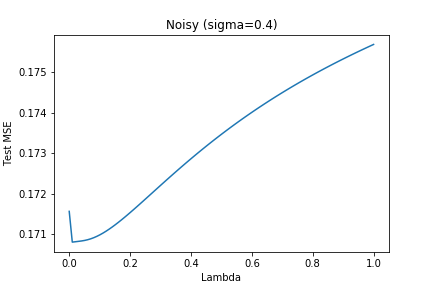
\includegraphics{figures/4_test_mse_noisy_ridge.png}
    \caption{Ridge regression on noisy data: Test MSE versus lambda}
    \label{}
\end{figure}
\section{Lasso regression on the Franke function with resampling}
Lasso regression is related to ridge regression in the sense that we try to minimize a penalized version of the sum of squared errors cost function. This time, we want our $\beta$ estimates to be

$$
\hat{\beta} = \argminA_{\beta} \left\|\mathbf{y - X\beta}\right\|^2 + \lambda\left\|\beta\right\|_1
$$

where $\left\|\beta\right\|_1 = \sum_{j=0}^{n}{|\beta_j}|$

Here, we do not have a closed-form solution of the minimization problem, and the parameters have to be optimized using gradient descent techniques. Instead of implementing these, we here rely on the \texttt{Lasso} class from \texttt{sklearn.linear\_model}. In the notebook \texttt{20191005-Lasso-regression-Franke.ipynb} we repeat most of the above Ridge regression analysis, this time using Lasso. Unfortunately, we are not able to get very interesting results here. The error seems to be growing with increasing values of lambda - meaning that Lasso in this case does not outperform Ordinary Least Squares. Maybe complicating the data further by adding even more noise could lead to more interesting results.

\section{Real data}
After having tested our methods for fitting and evaluation on generated datasets, we are now ready to work with real data\footnote{The assignment text seems to imply that all the analysis we did on the generated data should be repeated at this point, but due to time shortage I will be rather brief in this section.}. We will try to model terrain data from a small part of Norway, as shown in the following figure:

\begin{figure}[h]
    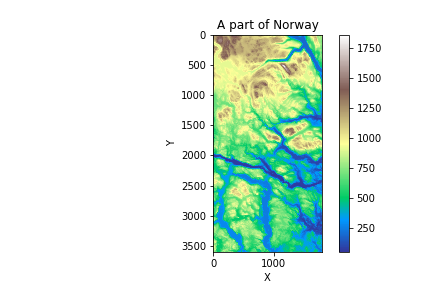
\includegraphics{figures/map}
    \caption{Plot of terrain data}
    \label{}
\end{figure}

In the notebook \texttt{20190907-introducing-terrain-data.ipynb} we scale the data using the \texttt{StandardScaler} class from \texttt{sklearn.preprocessing}. In order to evaluate the models we obtain, we here choose to use \texttt{train\_test\_split} from \texttt{sklearn.model\_selection}. We transform the input data into a feature matrix and slice it in order to obtain polynomial fits ranging from degree=1 (linear) to degree=8. Using the OLS method, we obtain the following test MSE scores and $R^2$ scores when evaluating on the test set:

\begin{table}[h!]
    \pgfplotstabletypeset[
        col sep=comma, ignore chars={, \%},
        precision=5,
        every head row/.style={
            before row={
                \hline
            },
            after row=\hline
        },
        every last row/.style={
            after row=\hline
        },
        columns/{0}/.style={column name=Degree, string type}
    ]{csv_files/6_mse_r2_score_ols_real_data.csv}
    \caption{MSE and $R^2$ score on terrain data, sorted by degree}
\end{table}

As we see, the error falls monotonically, but flattens somewhat as the degree becomes higher. Of course we could try fitting polynomials with a degree higher than 8, but the table above seems to imply that we would not get much of an improvement. The $R^2$ scores are far from 1, but at least they reveal that around half of the variability in the data is explained by a eight-degree polynomial model.

In the same notebook, we also try out Ridge regression and Lasso regression. In order not to have too many different datasets, we concentrate on the eight-degree variation, which had the least test MSE when performing ordinary least squares regression. Ridge regression seems to lead to increasing MSE with increasing values of lambda, and as for Lasso, the algorithm has problems converging. In an ideal world, this should have been investigated further.

\section*{Conclusion}
In this project, we have performed different variations on regression analysis, both generated data (with or without noise) and real world data. We have also discussed methods for evaluating how well our methods perform. In the cases we have investigated, it seems Ordinary Least Squares regression performs at least as well as the regularized versions (Ridge and Lasso regression.) The only possible exception is with the noisy dataset (Figure 3), where Ridge regression maybe could lead to a slight improvement. Figure 2 however seems to confirm beyond doubt that test MSE actually may be lowered by decreasing the complexity of the models.

One principal problem with the approach followed in this project is that the hyperparameters - both the degree of the polynomials and the $\lambda$ parameter in Ridge and Lasso regression - are chosen in a somewhat capricious manner. This should be done much more systematically in order to obtain reliable results. To a certain degree, this may be done using for instance \texttt{sklearn.model\_selection.GridSearchCV}.

There are of course other regression approaches that could be tried out too, like tree-based regression. And there are data transformations - like Principal Components Analysis - that could reduce the dimensionality of the input data, thereby increasing the predictive power of our models. As was stated initially, reproducibility has been a chief aim in shaping the overall structure of this project. But just as all science should have a firm grounding in the data and sources on which it is based, it should also point towards new investigations, and is it is hoped that the notebook-oriented approach adopted here not only facilitates reproducibility, but also expandability, in the sense that new methods and data can be easily integrated into the existing structure.

\begin{thebibliography}{3}
    \bibitem{geron}
    Aur\'elien G\'eron.
    \textit{Hands-On Machine Learning with Scikit-Learn and TensorFlow}
    O'Reilly, 2017

    \bibitem{introduction}
    Gareth James, Daniela Witten, Trevor Hastie, Robert Tibhirani.
    \textit{An Introduction to Statistical Learning}
    Springer, 2013

    \bibitem{elements}
    Trevor Hastie, Robert Tibshirani, Jerome Friedman.
    \textit{The Elements of Statistical Learning}
    Springer, 2009
\end{thebibliography}
\end{document}
